\documentclass[10pt]{proc}

\usepackage{amsmath}    % need for subequations
\usepackage{graphicx}   % need for figures
\usepackage{verbatim}   % useful for program listings
\usepackage{color}      % use if color is used in text
\usepackage{subfigure}  % use for side-by-side figures
\usepackage{hyperref}   % use for hypertext links, including those to external documents and URLs
\usepackage{multicol}
\usepackage{textcomp}

\author{P.~Gusev, J.~Burke}
\title{NDN-RTC Technical Report (draft)}

\begin{document}

\maketitle

%************************************************
\abstract
TBD

%************************************************
\section{Introduction}
TBD

%************************************************
\section{Background and prior work}
TBD

%************************************************
\section{Goals}
TBD

Goals:

\begin{itemize}
\item Low-latency (150-300ms) audio/video communication
\item Multi-party conferencing
\item Passive consumer (no negotiation and/or coordination)
\item Content verification
\end{itemize}

%************************************************
\section{Architecture}
There are two main roles defined in NDN-RTC: producer and consumer. In presence of NDN network the paradigm of real-time communication shifts from the push-based (when producer writes data to the socket and consumer reads it as fast as possible) to the pull-based (producer publishes data on the network with his own pace, while consumer has to request the data he needs and manage incoming data segments).
Producer's main task is to grab media data from media inputs, encode it, pack into network packets and store them in the cache. A lifetime for the data should be also defined by a producer (data freshness period).

Consumer implements more sophisticated algorithms for achieving the following goals:
\begin{itemize}
\item ensure fetching the latest data from the network; 
\item monitor network conditions and choose appropriate bandwith from a selection provided by a producer;  
\item playback fetched media in correct order;
\item handle network latency and packet drops.
\end{itemize}

\begin{figure}[Ht!]
\centering
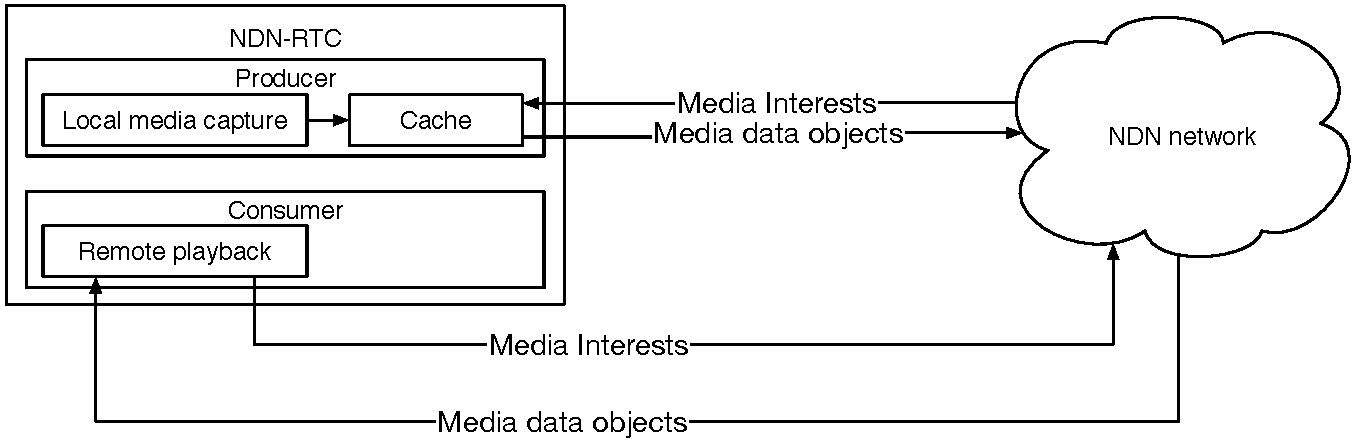
\includegraphics[width=0.5\textwidth]{architecture}
\caption{RTC over NDN}
\label{fig:arc}
\end{figure}

Figure \ref{fig:arc} presents top-level overview of how NDN-RTC works. Local media capture and Cache belong to the producer part of the NDN-RTC. Media is stored in the cache which provides access to the data for all incoming interests. Remote playback represents consumer: it issues interests, prepares received media (assembles video frames from segments and re-orders them) and plays it back.

\paragraph{Producer}

In case of video streaming, producer uses video encoding in order to reduce size of the frames. There are two types of frames used for encoding: \textit{Key} frames and \textit{Delta} frames. Key frames contain the most of the video information and don't depend on any previous frames to be decoded. Whereas Delta frames are dependent on all previous frames received after the last Key frame and can't be decoded without significant visual artifacts if any of those frames are missing.

Encoded frames vary in size, but average bitrate stays the same. For example, these are the sizes of frames for 1000 kbps stream:
\begin{itemize}
\item \textbf{Key frames} $\approx$ 30KB;
\item \textbf{Delta frames} $\approx$ 3-7KB.
\end{itemize}

Therefore, depending on the underlying internet protocol used (IP in the existing NDN testbed), producer may need to segment encoded frames into a smaller chunks and provide clear naming conventions for consumer to fetch them (see Figure \ref{fig:producer}).

\begin{figure}[Ht!]
\centering
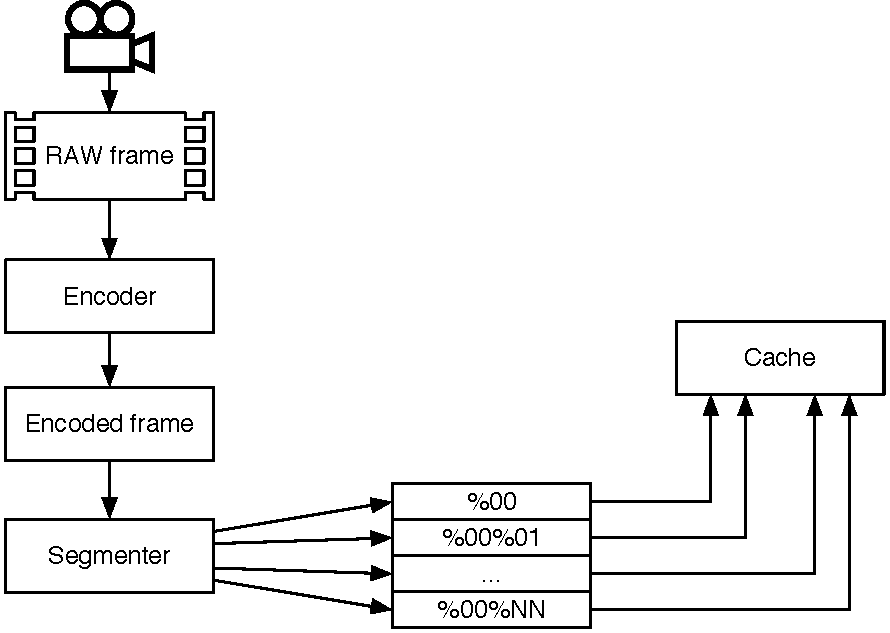
\includegraphics[width=0.5\textwidth]{producer}
\caption{NDN-RTC producer}
\label{fig:producer}
\end{figure}

\paragraph{Consumer}

Consumer takes into account that media packets are presented by separate segments in the network. Therefore, consumer implements mechanisms of interest pipelining and frame buffering (see Figure \ref{fig:consumer}). Interest pipeliner issues interests for individual segments and is controlled by some higher-level logic which achieves one out of four consumer's goals - ensures that only the latest data is fetched. Packets re-ordering, drops and latency fluctuations absorbtion are attained by the frame buffer which introduces buffering delay and arranges received frames in the playback order.

\begin{figure}[Ht!]
\centering
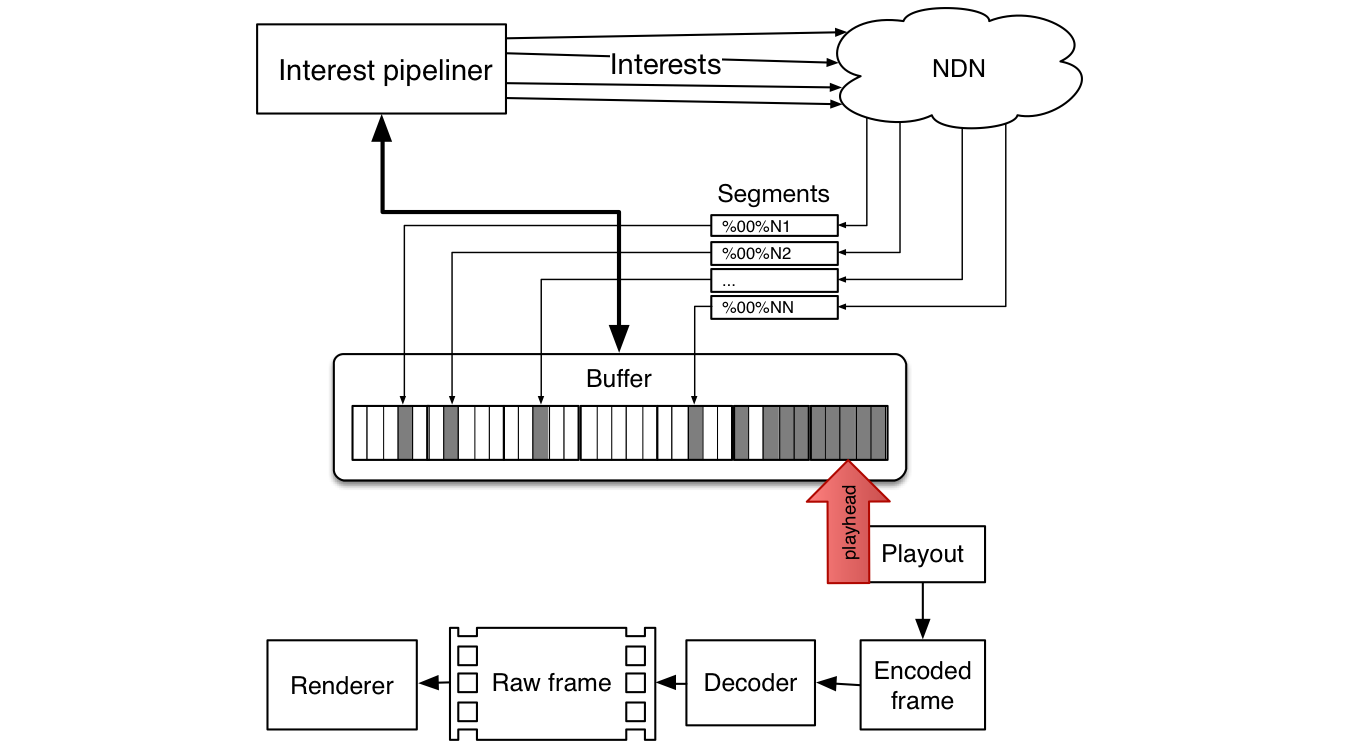
\includegraphics[width=0.5\textwidth]{consumer}
\caption{NDN-RTC consumer}
\label{fig:consumer}
\end{figure}


%************************************************
\subsection{Namespace}

As there is no direct consumer-produder communication, it is producer's job to provide as much supportive information as possible so that consumer is able to use this information in order to achieve her goals. There are several kinds of data producer can publish and these kinds should be reflected in the namespace:

\begin{itemize}
\item Media data
\begin{itemize}
\item Video frames
\item Audio samples
\end{itemize}
\item Forward error correction data
\item Producer's streams meta info
\end{itemize}

Besides that, the namespace should also reflect data specialization hierarchy - from general concepts in the root to more specialized entities towards the leaves. 

NDN-RTC producer uses a concept of \textit{media stream} for describing published media. Media stream represents a flow of raw media packets (video frames or audio samples) coming from an input device. Streams usually derive names from their input devices. It is quite natural for a producer to publish several media streams simultaneously, if she has more than one device to publish media from (for instance, publish video from camera, audio from microphone and another video stream for sharing computer screen). As all raw data should be encoded, the next level in the name hierarchy represents different encoder instances called \textit{media threads}. Thus, media threads allow producer to provide same media stream in several copies, for instance in low, medium and high quality for video, so that consumer can have a chance to choose media thread more suitable for the current network conditions.

\begin{figure}[Ht!]
\centering
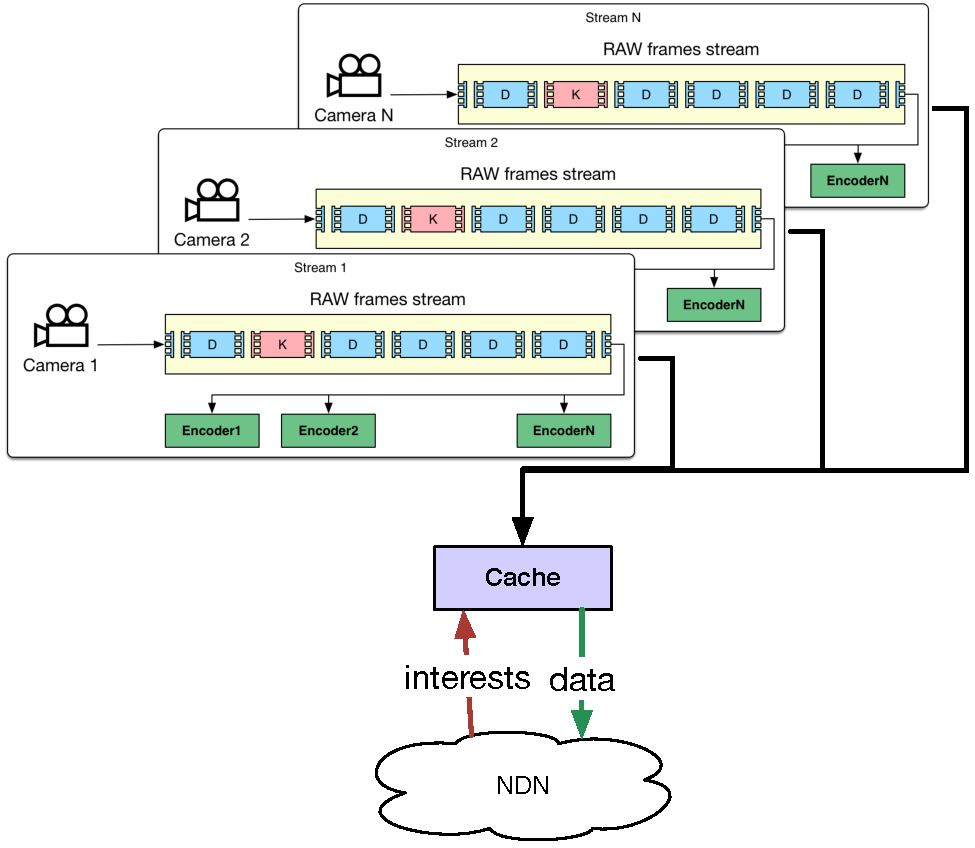
\includegraphics[width=0.5\textwidth]{streams-hierarchy}
\caption{NDN-RTC media streams hierarchy}
\label{fig:stream-hierarchy}
\end{figure}

NDN-RTC does not use any specific media container format for delivering its media to consumers. Instead, encoded media packets are segmented if needed and published under distinctive hierarchical names. Video frames are separated into two domains as per frame type: \textit{delta} and \textit{key} and numbered sequentially and independently. Both sequence numbers for delta and key frames start from 0. Next level specializes data type - it can be either media data or parity. Parity data, if producer opts to publish it, can be used by consumer to recover frames that miss one or more segments. The topmost level of the namespace defines individual data segments. These segments are also numbered suquentially and segment numbers conform to NDN naming conventions \cite{ndn_naming}.

There are some differences in case of the audio streams. First, there are no key frames, therefore all the audio packets are published under the \textit{delta} namespace. Second, audio samples are significantly smaller than video frames and do not require to be segmented. In practice, it appears that multiple audio samples can be bundled into one data segment. Therefore, instead of segmenting audio packets, they are bundled together until the size of one data segment is reached and published only after that.

Consumers need to know producer's streams structure in order to fetch data successfully. In order to save consumer from traversing actual producer's name tree, which can be time-consuming and unreliable, producer publishes meta information about her current streams under \textit{session info} component. Thus, consumers can retrieve up-to-date information about the producer's state.

\begin{figure}[Ht!]
\centering
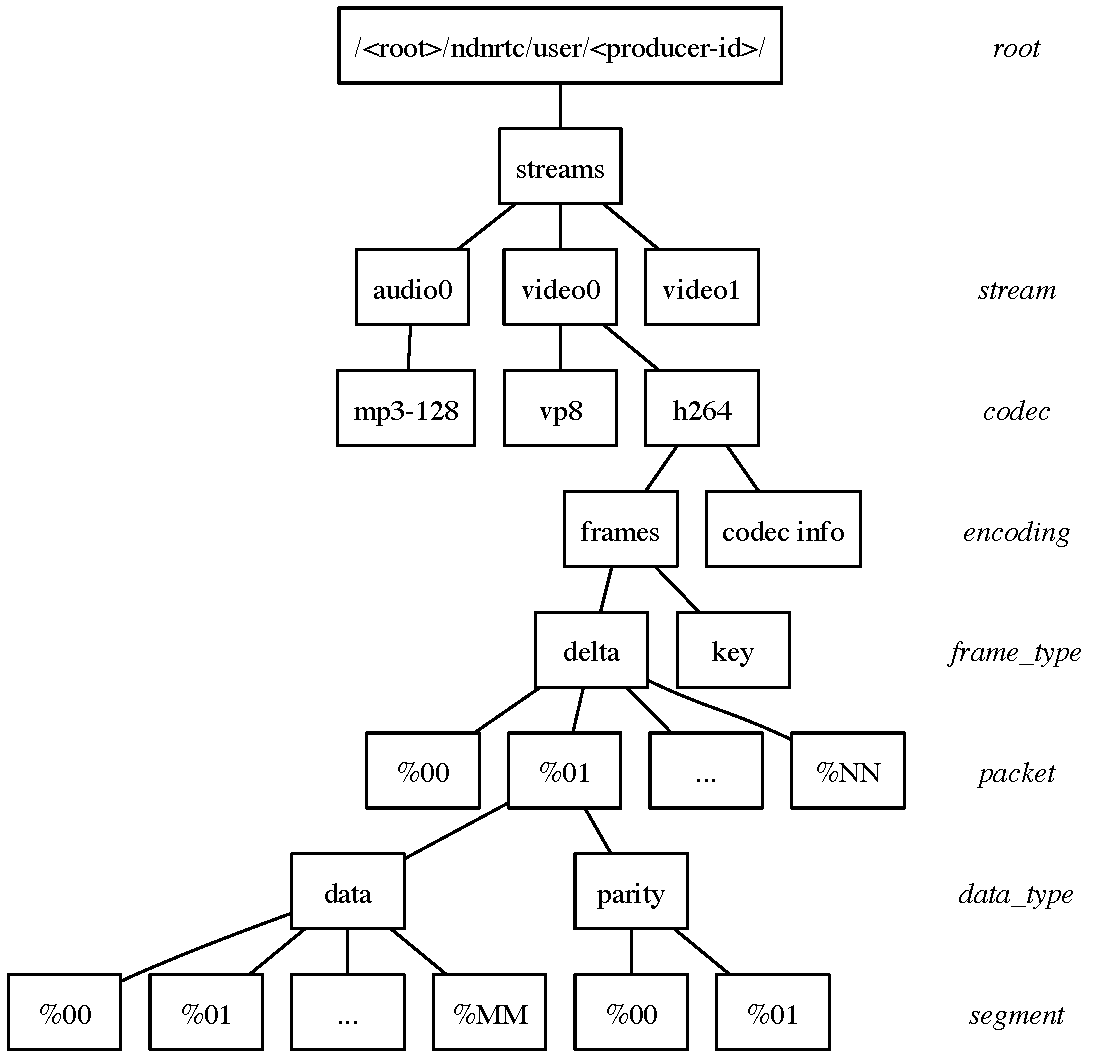
\includegraphics[width=0.5\textwidth]{namespace}
\caption{NDN-RTC namespace}
\label{fig:namespace}
\end{figure}

Besides naming data objects, data names can be appended by some additional media-level meta information which can be utlilized by consumers regardless of which frame segment was received first. Three components are added at the end of every data segment name:
\small\begin{equation}
.../\textbf{segment\#}/\textbf{playback\#}/\textbf{paired\_seq\#}/\textbf{num\_parity} \nonumber
\end{equation}\normalsize
\begin{itemize}
\item \textit{playback\#} - absolute playback number for current frame; this is different from the \textit{frame\#} which is a sequential number for the frame in its' domain (i.e. Key or Delta);
\item \textit{paired\_seq\#} - sequential number of the corresponding frame from other domain (i.e. for delta frames, it is sequential number of the corresponding key frame which is required for decoding);
\item \textit{num\_parity} - number of parity segments for this particular frame.
\end{itemize}


%************************************************
\subsection{Data objects}
Producer generates signed data objects from input media streams and places them in cache instantly. Incoming interests retrieve data from cache, if it is present, or forwarded further to the producer, if the requested data has not been produced yet. In such cases, producer maintains a pending interests table (PIT), which is checked every time new data object is generated. If an interest for newly generated data object exists in the PIT, it gets answered and PIT entry is erased.

Besides actual stream data, data objects contain some amount of meta information which is prepended during frames segmenting (see Figure \ref{fig:segment}). There are two types of headers: \textit{Frame header} and \textit{Segment header}. Frame header is prepended to segment \#0 of each individual video frame and contains media-specific information (such as size of a frame), timestamp, current rate and unix timestamp, which can be used for calculating actual delay between NTP-synchronized producer and consumers (see Figure \ref{fig:data-struct}). Segment header is prepended to every segment of a frame. It carries network-level information which can be used by consumer for making certain assumptions about current network conditions and origin of the data objects received:
\begin{itemize}
\item Interest nonce

Nonce value of the interest which requested this particular segment. There are three meaningful cases: 
\begin{itemize}
\item \textit{value belongs to the interest issued previously} - consumer received non-cached data requested by interest issued previously;
\item \textit{value is non-zero, but doesn't belong to any of the previously issued interests} - consumer received data requested by some other consumer; data may be cached;
\item \textit{value is zero} - consumer received data which was cached on producer side and never requested by anyone before.
\end{itemize}

\item Interest arrival timestamp

Timestamp of the interest arrival. Monitoring this value and interest expression timestamps over time may give consumer a clue about how long does it take for interests to reach producer. This value is only valid when nonce value belongs to one of the consumer's interests.

\item Generation delay

Time interval in milliseconds between interest arrival and segment publishing. Consumer can use this value to her advantage in order to control the number of outstanding interests. This value is only valid when nonce value belongs to one of the consumer's interests.

\end{itemize}

\begin{figure}[Ht!]
\centering
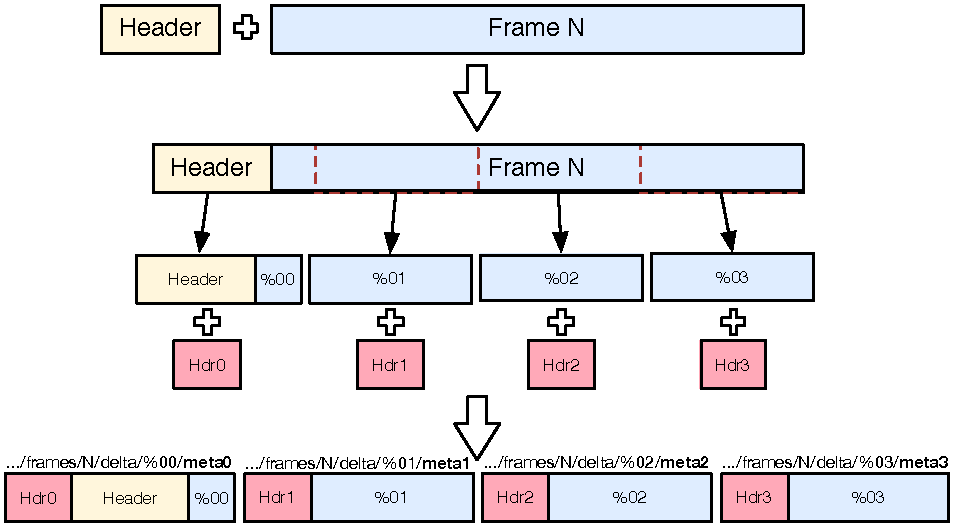
\includegraphics[width=0.5\textwidth]{segmentation}
\caption{Frame segmentation}
\label{fig:segment}
\end{figure}

\begin{figure}[Ht!]
\centering
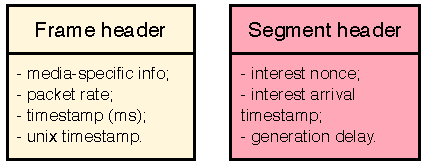
\includegraphics[width=0.3\textwidth]{data-struct}
\caption{Frame and segment headers}
\label{fig:data-struct}
\end{figure}

Audio samples are not prepended by any segment header, however the whole audio bundle is prepended by the same frame header (see Figure \ref{fig:audio-bundling}).

\begin{figure}[Ht!]
\centering
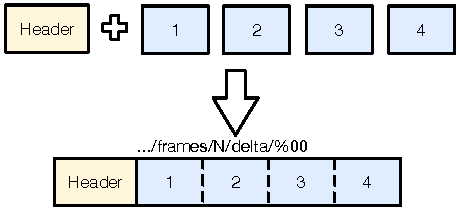
\includegraphics[width=0.3\textwidth]{audio-bundling}
\caption{Audio bundling}
\label{fig:audio-bundling}
\end{figure}


%************************************************
\subsection{Consumer protocol}

%************************************************
\subsubsection{Frame fetching}

Consumer doesn't know the total number of segments beforehand, unless the very first segment is fetched - in this case, consumer can retrieve metadata from the received segment and get total number of segments for the current frame. 
Therefore, at first attempt, consumer tries to make a "best guess" in the number of segments she needs to fetch by issuing $M$ interests (see Figure \ref{fig:pull}). If interests arrive too early, they will be added to the producer's PIT and stay there for some amount of time $d_{gen}$ called \texttt{generation delay}. Once encoded frame is segmented into $N$ segments and these segments are published, interests $0 - M$ are answered with the data which travels back to consumer. Upon receiving first data segment, consumer retrieves metadata from it and determines total number of segments for current frame. In case if $N > M$, consumer issues $N - M$ more interests for the missing segments. These segments will be satisfied by data with no generation delay (as the frame has been published already by producer). The time interval between receiving very first segment and until the frame is fully assembled is represented by $d_{asm}$ and called \texttt{assembling time}.

\begin{figure}[Ht!]
\centering
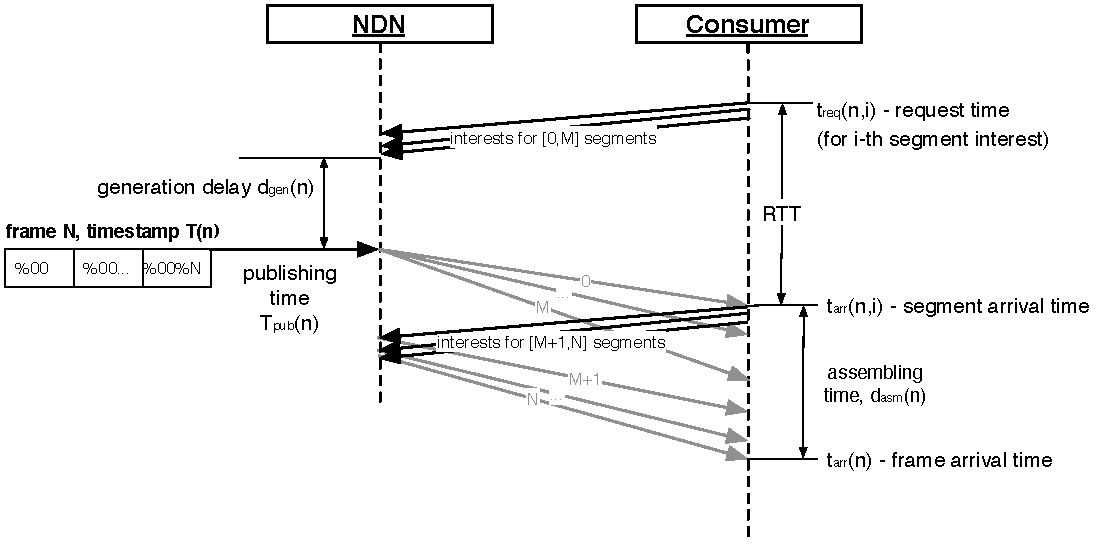
\includegraphics[width=0.5\textwidth]{frame-fetch}
\caption{Fetching frame}
\label{fig:pull}
\end{figure}

It is needlesss to say, that additional round-trips for requesting missing data segments increase overall frame assembling time and chances that the frame will be incomplete by the time it should be played back. This problem could have been avoided if consumer could make a better guesses in the number of initial interests. Therefore, the following considerations were introduced in later versions of the library:
\begin{itemize}
\item consumer should know what type of frame she is going to fetch (as average number of segments varies greatly for different frame types);
\item consumer should track average number of segments per frame type.
\end{itemize}

The first consideration was implemented by introducing separate namespaces for key and delta frames. The second consideration helps consumer do better at guessing the number of initial interests.

\subsubsection{Bufferization}

% Buffer:
% - re-ordering
% - added latency to mitigate network delays
% - extended defition:
% 	- pending frames
% 	- assembling frames
% - buffer-based retransmissions

As in traditional streaming applications, consumer uses frame bufferization in order to tackle out-of-order data arrivals and network delay deviations. Consumer-side jitter buffer is also used as a place for assembling frames by segments. However, the definition of jitter buffer is extended for NDN networks. In traditional push-based approach, buffer can not contain empty frame slots - they are allocated/reserved only when data arrives. Pull-based paradigm requires consumer to request data explicitly. Therefore an after expressing interest consumer "knows" that new data is coming and a frame slot should be reserved in the buffer. Practically, this means, that there will always be some number of empty reserved slots in the buffer. Therefore, jitter buffer's size have two measurements:
\begin{itemize} 
\item \textit{playback size} - playback duration of all complete ordered frames by the moment;
\item \textit{estimated size} = \textit{playback size} + \textit{number of reserved slots} $\times$ 1/\textit{producer rate}
\end{itemize}

% Pull-based one-to-many media data fetching results in different bufferization mechanisms for the consumer. Consumer should be aware that the data requested could not come earlier than the RTT value for the current network topology (see Figure \ref{fig:pull}), assuming that data has been already placed in the content store of a forwarder by the time it received the interest. Moreover, RTT values can vary greatly (order of magnitude) depending on how far in the network interest should go (in case there are several hubs between consumer and producer). Clearly, consumer should be aware of this fact and take this into consideration while performing measurements. However for now, we assume that RTT values will not vary greatly.

% Consumer is interested in getting the most recent data from the network. Taking into account RTT value, consumer should express interests in such a way, that they could arrive to the producer as close as possible to the frame publishing time $T^{pub}_{n}$. In general, RTT value for the $i$-th interest of the $N$-th frame can be expressed by the following equation:
% \begin{equation}
% RTT_{ni} = t^{arr}_{ni} - t^{req}_{ni}
% \end{equation}
% where $t^{req}_{ni}$ - timestamp when the interest for $i$-th segment of $N$-th frame was expressed, $t^{arr}_{ni}$ - timestamp when the $i$-th data segment of $N$-th frame was received.

% From the other point of view, RTT value can be represented like this:
% \begin{equation}
% RTT_{ni} = \widehat{RTT} + d^{gen}_{ni} + w_i
% \end{equation}
% where $\widehat{RTT}$ - real RTT value for the current network conditions, $d^{gen}_{ni}$ - delay between the moments when the interest has reached producer and requested data has been added to the content store, $w_i$ - network-introduced delay.
% Whereas $w_i$ component cannot be omited entirely (though can be tracked), $d^{gen}$ is the variable that should be minimized by consumer in order to get the most accurate RTT estimation for the current network. 

% Knowing RTT value is important for the consumer due to several reasons:

% \begin{itemize}
% \item consumer can estimate which fame number to request in order to get the latest data;
% \item consumer can track segments arrival and set a deadline when a frame should be assembled and re-express interests for missing segments so that they can still arrive in time in order to finalize the frame.
% \end{itemize} 

% As network does not guarantee packet delivery, consumer should be aware of data losses and incorporate this knowledge in bufferization mechanisms. 

% Proposed frame buffer is presented on Figure \ref{fig:buffer}. This is a circular buffer with frames being assembled while moving from the left side (beginning) to the right side (end) of the buffer. New frames (recently requested by issuing interests) enter buffer in the beginning of the buffer and exit in the end of the buffer. Further, we will analyse and measure different frame positions inside the buffer using time scale (milliseconds), i.e. if the buffer size is $B$ milliseconds, then the frame $F_n$ which should be played back at the time $t_n$ has entered the buffer at the time $t_n-B$.

% In order to understand, how buffer size should be determined, let's apply reasoning, explained in next paragraph.

% To handle data losses, buffer needs a retransmission check point at which interests for the missing frame segments can be re-expressed. This checkpoint should be placed far enough from the point when the frame should be played back so the missing data could arrive by this time. Any expressed interest is expected to bring data segment in $\overline{RTT}$ milliseconds (where $\overline{RTT}$ - consumer's estimation of the current RTT value). Therefore, retransmission checkpoint should be placed at least $\overline{RTT}$ milliseconds earlier before the end of the buffer (playback deadline). The same reasoning could be applied to determine a point in time at which initial interests should be expressed (i.e. beginning of the buffer). In ideal network conditions (with no losses), re-transmission of interests for missing segments should not be required, i.e.  frame should have been already assembled by the time of retransmission checkpoint. This means that the point of time for initial interests issuing should be placed $\overline{RTT}+\overline{d^{asm}}$ milliseconds earlier than retransmission checkpoint, where $\overline{d^{asm}}$ - is the observed average assembling time for this specific frame type (as it can vary greatly depending on frame type - Key or Delta). Therefore, according to the Figure \ref{fig:buffer}, the values of $P$ (pipeline size of the buffer) and $J$ (jitter size of the buffer) should satisfy these inequalities:

% \begin{equation}
% P \geq \overline{RTT} + \overline{d^{asm}}; J \geq \overline{RTT}
% \end{equation}


% \begin{figure}[Ht!]
% \centering
% 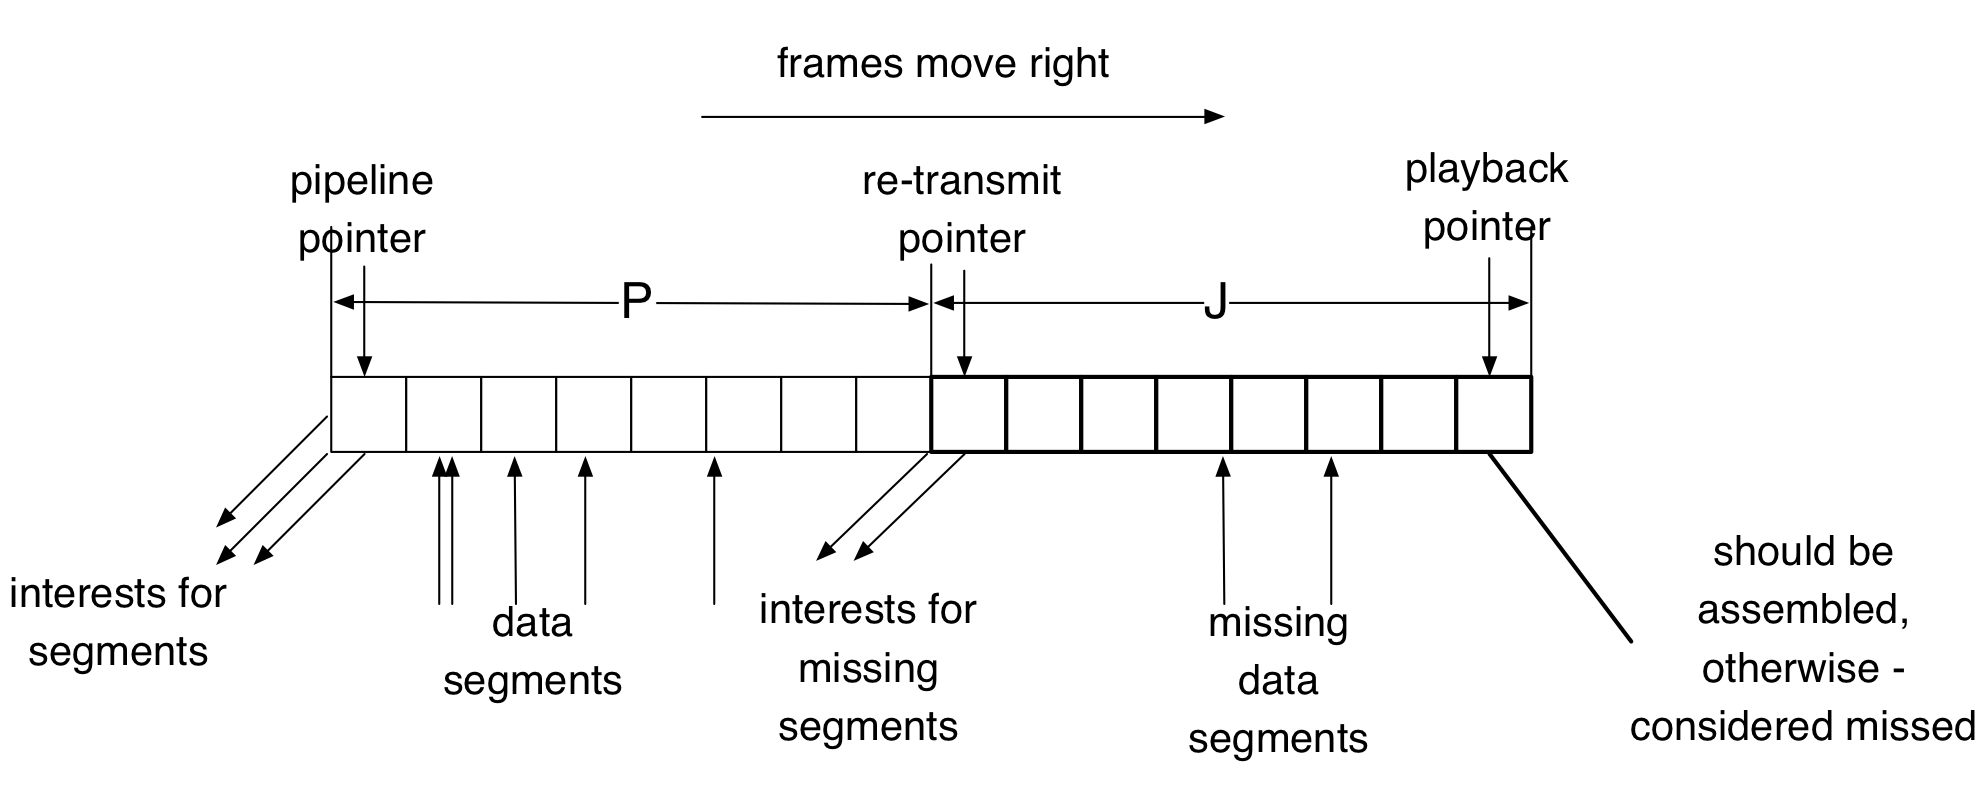
\includegraphics[width=0.5\textwidth]{buffer}
% \caption{Frame buffer}
% \label{fig:buffer}
% \end{figure} 

\subsubsection{Fetching process}
TBD

% NDN provides data caching which helps distributing server loads. On the other side, in case of many-to-many real-time communications fetching fresh data may be critical. 
% Before consumer can start playing back received media, she has to ensure that she has got the latest data from the network, i.e. old cached content should not be presented to the user. Therefore, consumer operates in two modes: 
% \begin{itemize}
% \item chasing mode 
% \item fetching mode
% \end{itemize}

% \paragraph{Chasing mode}
% Consumer switches into chasing mode in two cases:
% \begin{enumerate}
% \item data fetching initiation
% \item no new data arrived for continuous time
% \end{enumerate}

% Consumer stays in chasing mode unless she \textit{receives the latest data from the producer}. When consumer starts fetching data by issuing interests, it can get old data (up to \textit{freshness} seconds old) which is not useful anymore. In order to "chase" producer, consumer starts issuing interests with frequency, much higher than the frequency of data being produced (frames per second for video or sample rate for audio). After that, consumer monitors $d_{arr}$ - arrival delay of first segments for each frame and analyzes this value:
% \begin{equation}
% d_{arr} = \left\{\begin{matrix}
% growing \rightarrow \mbox{continue Chasing mode}\\ 
% stable \rightarrow \mbox{switch to Fetching mode}
% \end{matrix}\right.
% \end{equation}

% This decision is based on a simple idea: \textit{if interests are issued faster than the data is produced and the data arrives with data generation frequency, then interests are issued for the data that has not been produced yet}. Therefore, consumer is getting most recent data from the network. Figure \ref{fig:darr} shows how $d_{arr}$ grows over time in chasing mode.

% \begin{figure}[Ht!]
% \centering
% 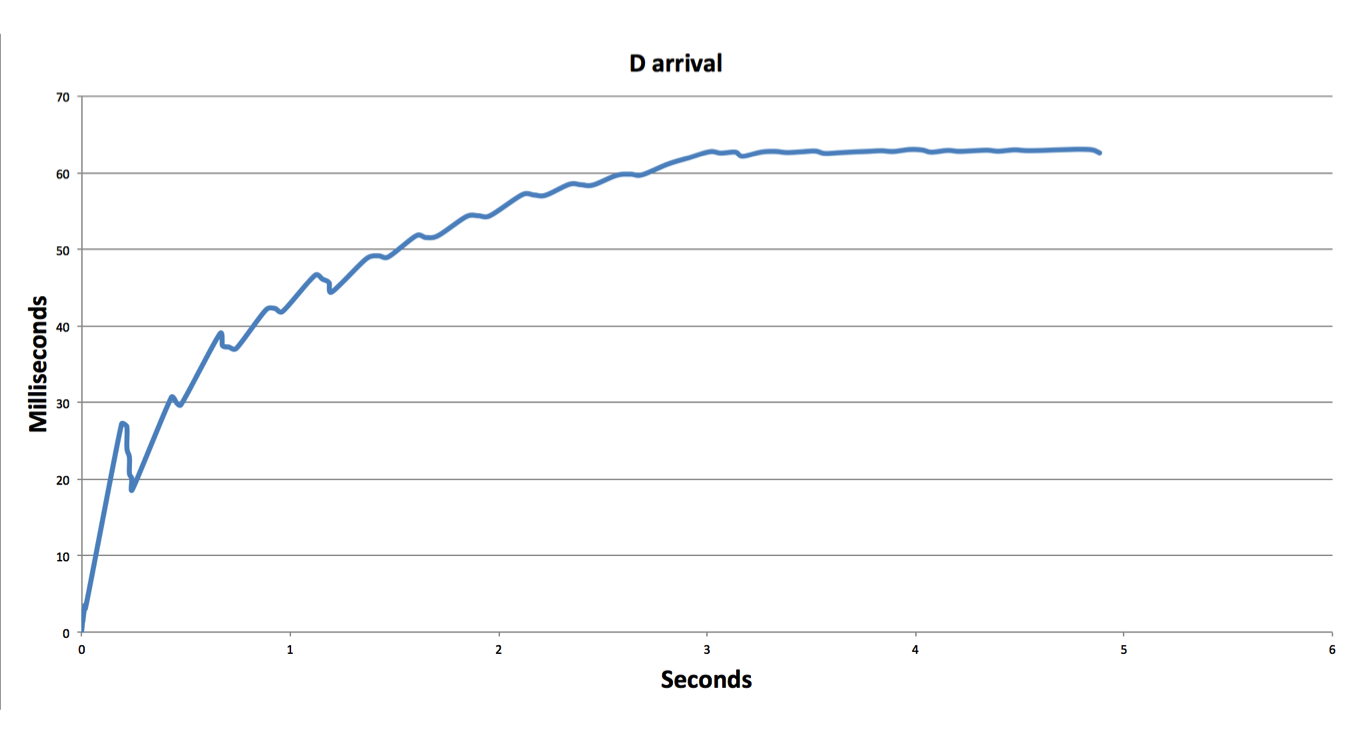
\includegraphics[width=0.5\textwidth]{darr}
% \caption{Data arrival delay $d_{arr}$ in chasing and fetching modes}
% \label{fig:darr}
% \end{figure} 

% \paragraph{Fetching mode}

% Once consumer concluded that she receives the lates data, she switches into fetching mode. In this mode, consumer's main task is to keep frame buffer size at the minimal required level (as was explained in the previous section - at least 2*$RTT$ seconds). Therefore, interest pipelining mechanism is controlled by the buffer - whenever buffer size becomes less than minimal buffer size, new interests are expressed unless buffer size returns to the required level. Since frames from the buffer are consumed at the playback rate, pipeliner mechanism expresses interests at least at the same rate.

% \subsubsection{RTT estimation}
% TBD

\section{Implementation}
TBD

\section{Evaluation}
TBD

\section{Issues and future work}
TBD

\section{Conclusion}

\end{document}